% !TEX root = main.tex

\section{Applications}

\subsection*{Problem description}

We will evaluate the results of the filters using the three-vortex problem~\cite{aref_motion_1979,yim_motion_2022}. This problem is analogous to the N-body problem in celestial mechanics. Starting with three bodies, Henri Poincaré demonstrated that these problems are sensitive to initial conditions, thus initiating the theory of modern chaos~\cite{poincare1890,diacu1996}.

Each vortex is positioned in a box of size $[0, \pi]^2$ and follows the distribution of the Bessel vortex~\cite{vanGeffen1996}. A Bessel vortex is defined by a continuous vorticity field on a circle of radius $R$ and is described by the equation

\begin{equation*}
    \omega(r) =  \begin{cases}
        \Gamma ~ J_0\left(\frac{k  r}{ R}\right),   \quad & r < R,        \\
        0 \quad                                           & \text{sinon},
    \end{cases}
\end{equation*}où $J_0$ is the first Bessel function, $k$ is its first non-trivial zero, $r$ is the distance from the center of the vortex, and $\Gamma$ is the vortex strength.

Independently, this is a stationary solution for the Euler equations in an infinite domain. In this case, each vortex rotates around its center with a constant angular velocity of $\frac{\Gamma}{2\pi}$ without changing shape. When multiple vortices are placed in a box, they begin to move due to the velocities induced by each other as well as the boundary conditions. Figure~\ref{sec
} shows the initial condition with the induced vorticity field and the trajectory of three vortices over time.

% Add the initial particle configuration
\begin{figure}~\label{sec
    }
    \centering
    \begin{subfigure}{0.5\textwidth}
        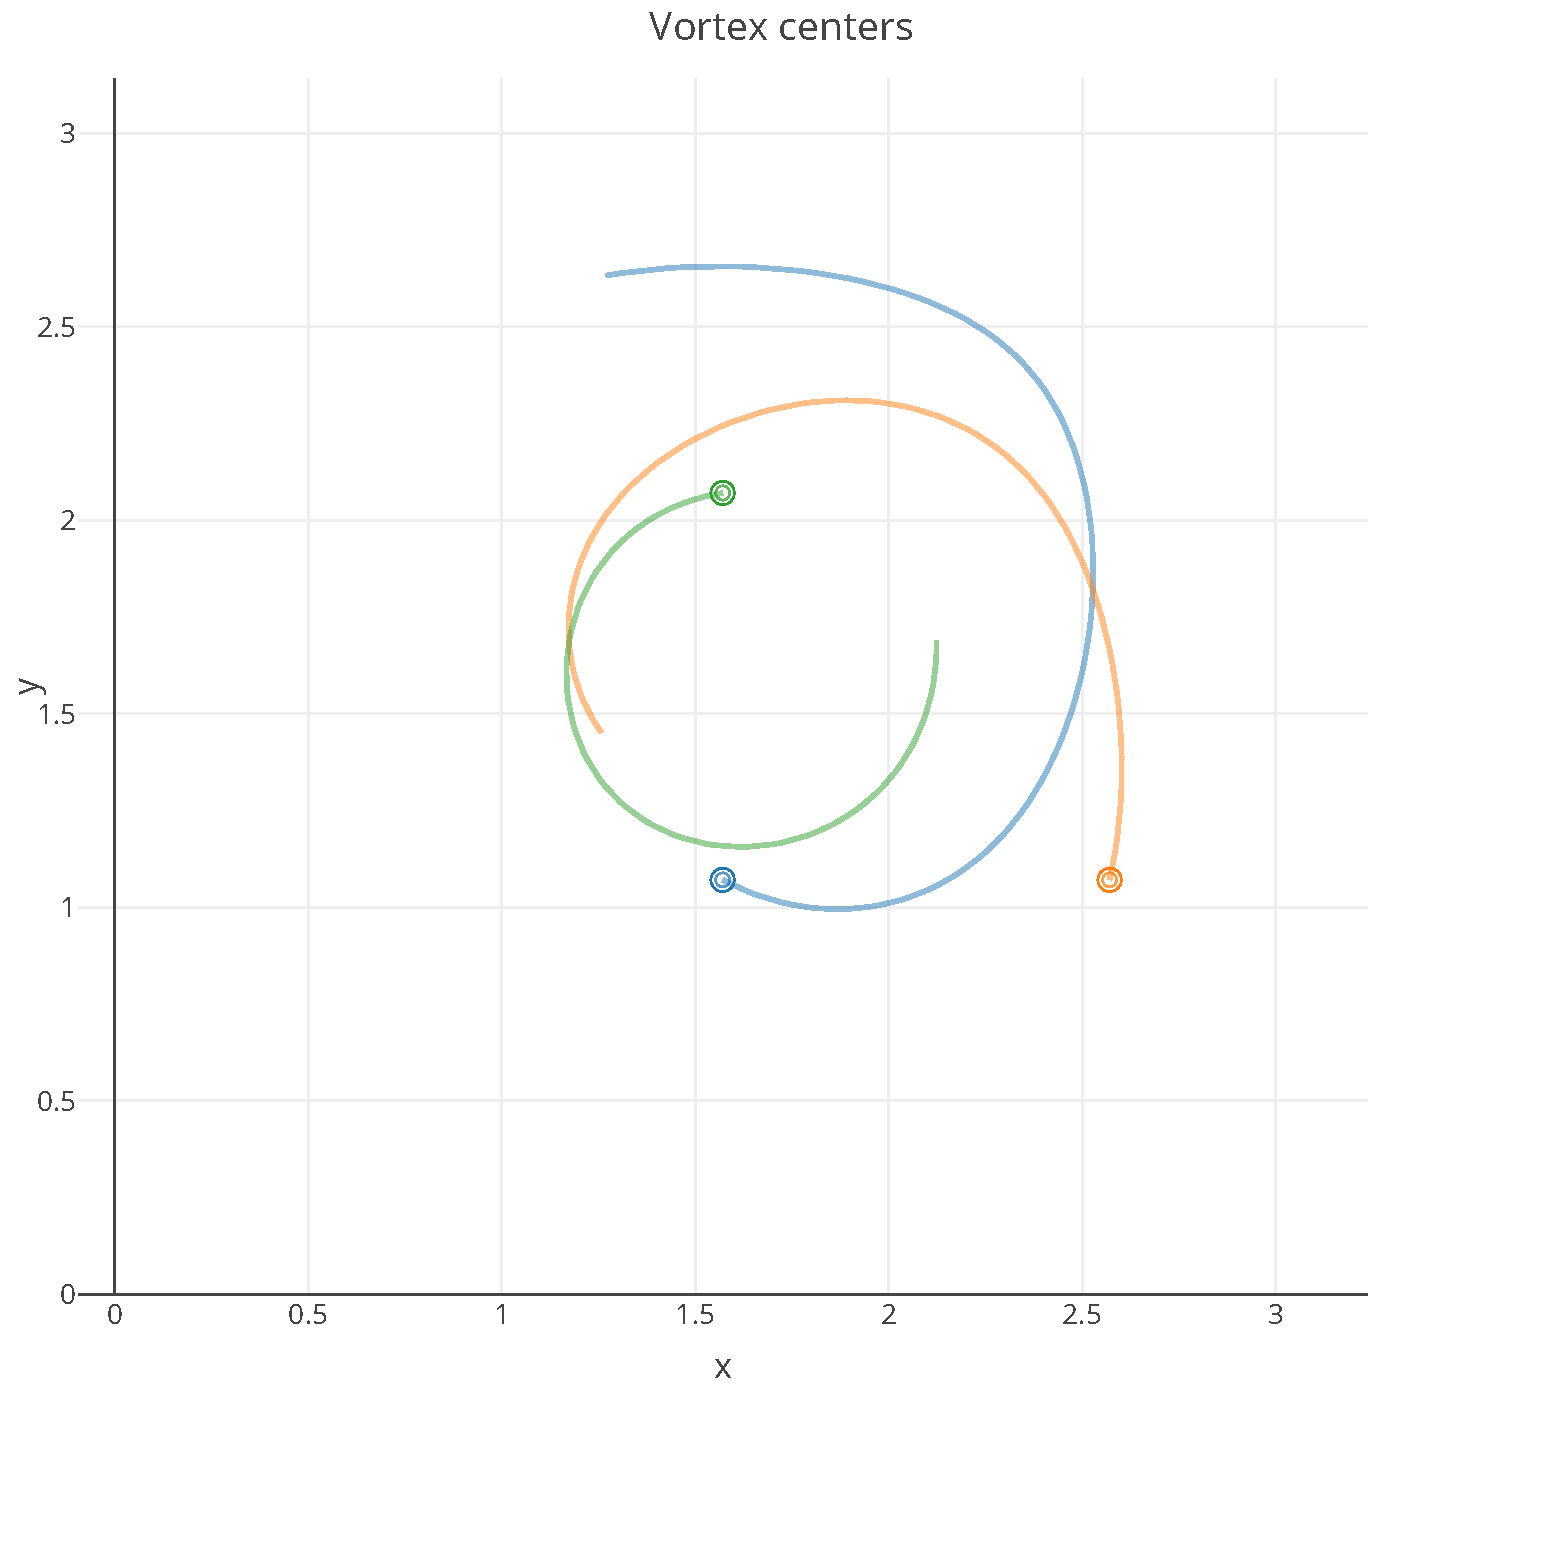
\includegraphics[width=\textwidth]{vortex_centers.pdf}
        \caption{Initiale particle configuration with induced velocity field.}
    \end{subfigure}
    \begin{subfigure}{0.5\textwidth}
        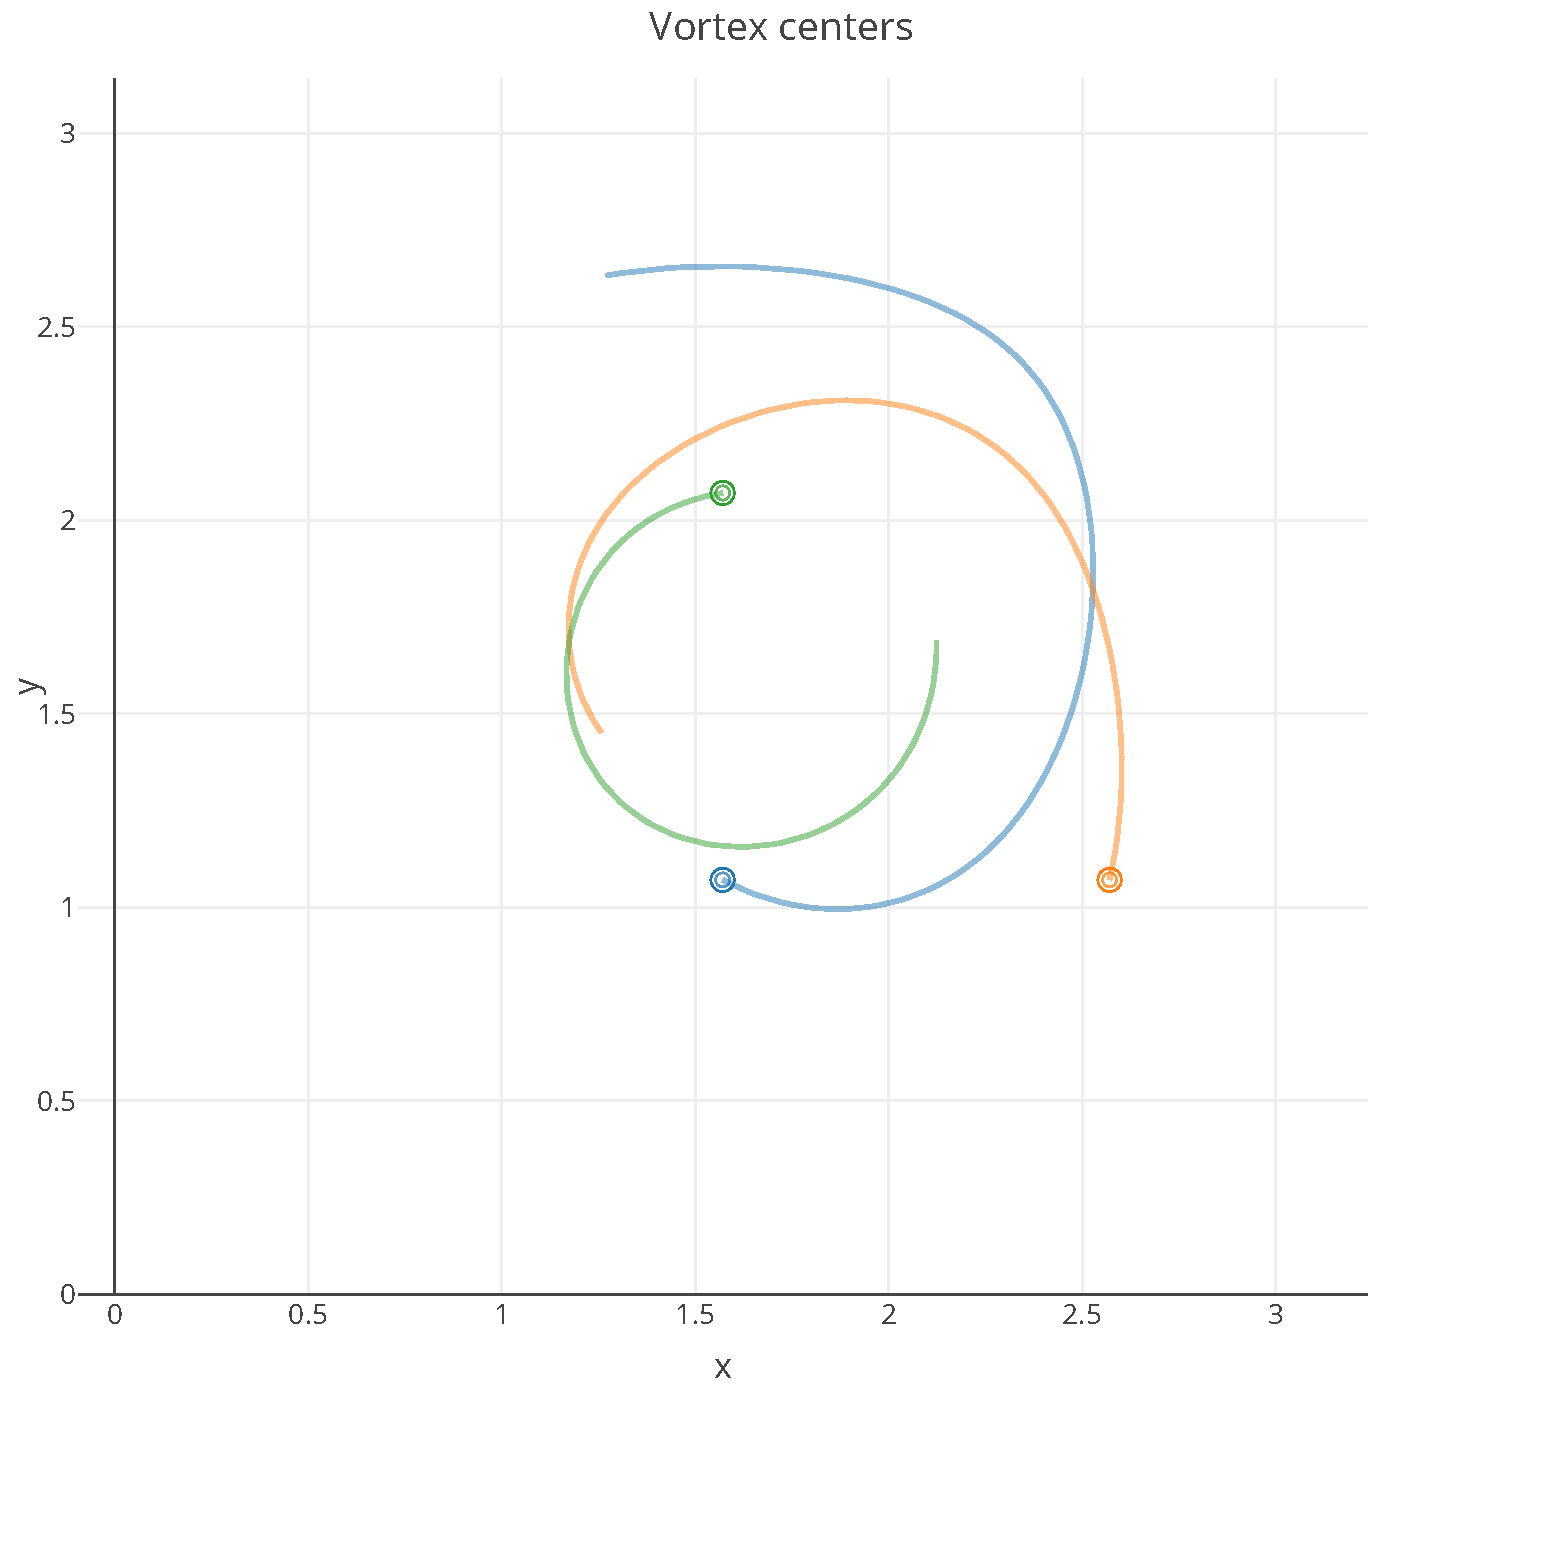
\includegraphics[width=\textwidth]{vortex_centers.pdf}
        \caption{Trajectory of the centers of three vortices over time.}
    \end{subfigure}
    \caption*{heading}
\end{figure}

\subsection*{Assimilation of vortex centers}

Due to the chaotic nature of the problem, a small perturbation in the initial conditions leads to an amplification of the error in the vortex trajectories.
We initially assume that the vortex centers, their size $R$,and their amplitude $\Gamma$ are known with an initial uncertainty, the values of which are reported in Table~\ref{tab:init_three_vortex}.The objective will be to track the positions of the three vortices.

\begin{table}[htbp]
    \centering
    \caption{Initial Conditions}
    \begin{tabular}[t]{|l|l|}
        \hline
        Variables            & Distributions \
        \hline
        Vortex center        & $\mathcal{N}(x^i,0.05^2), \quad \mathcal{N}(y^i,0.05^2) \quad i = {1,2,3}$ \
        Core size ($R$)      & $\mathcal{N}(0.2, 0.01^2)$ \
        Amplitude ($\Gamma$) & $\mathcal{N}(4.0, 0.08^2)$ \
        \hline
    \end{tabular}
    \label{tab:ref_three_vortex}
\end{table}

We assume different test case depending on the source of uncertainties :
\begin{itemize}
    \item Case 1: Position-only Uncertainty case. We assume that the core size and amplitude of the vortices are known precisely, while the positions of the vortices are subject to uncertainty ;\\
    \item Case 2: Position and Amplitude Uncertainty case. For the Position and Amplitude Uncertainty Case, both the vortex centers and their amplitudes are uncertain. The details of these uncertainties are provided in Table
\end{itemize}

The objective of these tests is to first separate the error arising from alignment (i.e., positional uncertainty) from the error due to intensity (i.e., amplitude uncertainty). By analyzing these cases individually, we aim to understand the distinct contributions of each type of uncertainty to the overall error in vortex trajectories and the ability to our different correction of assimilation.

For our observations, we use a noisy coarse grid with dimensions $N_{\text{obs.}} = 24\times 24$ points to measure velocity. The observed velocity components are supposed independent and affected by a noise, characterized by a standard deviation denoted as $\sigma_{\text{obs}}$ as illustrate in Figure~\ref{fig:observation}. This noisy velocity grid provides a practical means to assess how uncertainties in the observations influence the tracking of vortex positions.

\begin{figure}
    \centering
    \includegraphics[width]{name}
\end{figure}
\subsection*{Alignment}

% Traiter du cas avec uniquement une erreur d'alignement des membres. Présenter alors une comparaison entre les filtres par correction d'intensité et les autres.

